
\documentclass[12pt]{article}
\usepackage[a4paper, margin=.30in]{geometry}
\usepackage{graphicx ,
            wrapfig,
            xcolor, 
            enumerate,
            amsmath,
			fontenc,
			tcolorbox
            }

\newcommand\headerMe[2]{\noindent{}#1\hfill#2}
\renewcommand{\thesection}{\Roman{section}}

\author{Zakaria HAOUZAN}
\date{\today}

\begin{document}
% headers --------------
\headerMe{Matière : Physique-Chimie}{Professeur : Zakaria HAOUZAN}\\
\headerMe{Unité : Travail Mécanique et Energie }{Établissement : Lycée SKHOR qualifiant}\\
\headerMe{Niveau : 2BAC-SM-X}{Heure : 5H}\\

% ------Content ________
\begin{center}

    \Large{Leçon $N^{\circ} 2 $: \color{red}Ondes mécaniques progressives périodiques. }
\end{center}


\section{Notion d’onde mécanique progressive périodique}
\subsection{Définition : }

\begin{wrapfigure}[5]{r}{0.15\textwidth}
	\vspace{-2cm}
	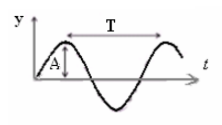
\includegraphics[width=0.15\textwidth]{./img/OMPsins.png}
	\caption{ onde mécanique périodique sinusoïdale}
\end{wrapfigure}

Une onde est périodique si elle se répète indentiquement à elle-même pendant des mêmes intervalles de temps appellés période T .  

Elle est dite sinusoïdale si sa variation est une sinusoïde en fonction du temps et l'élongation d'un point du milieu de propagation
s'écrit de la manière suivante: \\$y(t) = Asin(\frac{2.\pi}{T}.t + \phi)$

\vspace{-0.4cm}
\begin{itemize}
\item y(t): l’élongation à un instant t en (m).
\item A : l'amplitude (élongation maximale ) en (m).
\item T : la période (périodicité temporaire) et la frequence  $\nu = \frac{1}{T}$ (Hz).
\item la phase à l'origine, elle se détermine à partir des conditions initiales (en rad).
\end{itemize}

\subsection{Exemple 1:Périodicité temporelle }
En produisant un son à l'aide d'un haut parleur lié à un générateur (GBF) devant un microphone lié à un oscilloscope on obtient
l'enregistrement suivant:
\begin{figure}[h]
	\begin{center}
		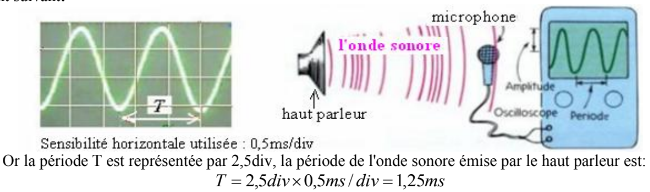
\includegraphics[width=0.6\textwidth]{./img/OMPPExemple1.png}
	\end{center}
\end{figure}
\begin{center}
	\vspace{-2.5cm}
\end{center}

\subsection{Exemple 2:Périodicité spatiale.}

La stroboscopie est une méthode d'observation d'un mouvement en utilisant le stroboscope qui est un appareil qui émet des éclairs
périodiques selon des fréquences réglables.
\begin{figure}[h]
	\begin{center}
	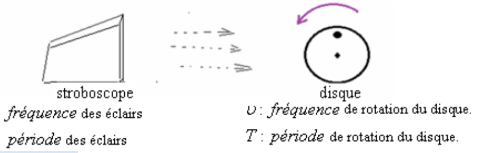
\includegraphics[width=0.5\textwidth]{./img/OMPPstroposcope.png}
\end{center}
\end{figure}

Durant la rotation le disque apparaît blanc, l'œil ne peut pas suivre le mouvement de la tâche et lorsqu'on l'éclaire avec le
stroboscope on s'intéresse aux trois cas suivants : \underline{l'immobilité apparente} et le mouvement apparent ralenti dans le même sens puis
celui dans le sens contraire du mouvement de rotation du disque et cela suivant les fréquences du stroboscope.

\textbf{\underline{Dans le cas de l'immobilité apparente :}}on observe que la tâche est immobile car elle est éclairée au même endroit.

\begin{figure}[h]
	\begin{center}
	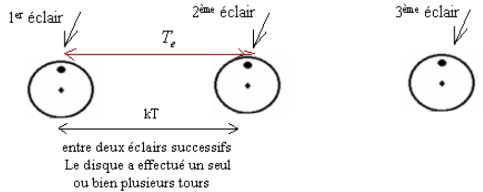
\includegraphics[width=0.5\textwidth]{./img/OMPPimmobilité apparente.png}
\end{center}
\vspace{-1.2cm}
\end{figure}

La relation entre la période des éclairs et celle de rotation du disque.$Te=kT$ avec $k\in N*$  donc $\nu = k\nu_e$

La plus grande fréquence des éclaires qui permet d'avoir l'immobilité apparente correspond à $k=1$ donc: $\nu=\nu_e$.

\textbf{\underline{Cas du mouvement ralenti apparent :}} -On obtient un mouvement ralenti apparent dans le même sens de rotation du disque si $\nu_e$ est est légèrement inférieure à $\nu$.

-On obtient un mouvement ralenti apparent dans le sens contraire de rotation du disque si $\nu_e$ est légèrement supérieure à $\nu$.

\section{Exemples d'ondes mécaniques progressives périodiques : }
\subsection{Onde progressive le long d'une corde : }
On utilise une corde élastique tendue horizontalement par un corps suspendu comme l'indique la figure suivante .La corde est attachée en S au bout d'une lame vibrante dont le mouvement est entretenu par un électro-aimant alimenté par un courant alternatif.

\begin{figure}[h]
	\begin{center}
\vspace{-0.5cm}
	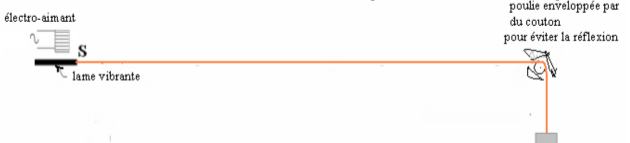
\includegraphics[width=0.66\textwidth]{./img/OMPPExperience.png}
\end{center}
\vspace{-2cm}
\end{figure}

Lorsque la lame vibre avec une fréquence $\nu = 100Hz$, la corde parait floue,ce qui prouve que tous ses points sont en mouvement.

En utilisant le stroboscope et en le réglant sur la fréquence $\nu_e = \nu =100Hz$, on obtient le mouvement apparent ralenti dans le sens contraire de celui de propagation de l'onde.
\begin{figure}[h]
	\begin{center}
\vspace{-0.5cm}
	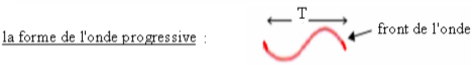
\includegraphics[width=0.46\textwidth]{./img/OMPPexProg.png}
\end{center}
\vspace{-1cm}
\end{figure}

\begin{wrapfigure}[10]{r}{0.27\textwidth}
	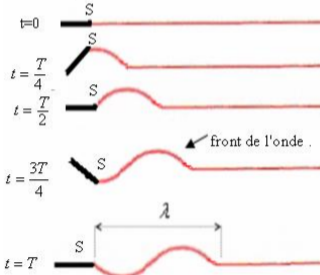
\includegraphics[width=0.29\textwidth]{./img/OMPPtimes.png}
\end{wrapfigure}


T: périodicité temporaire (période de l'onde progressive)

Faisons des représentations successives de l'aspect de la corde pendant des intervalles de temps successifs et égaux à T/4 (T étant la période de vibration de la source) :
$\lambda $: Longueur d'onde (périodicité spatiale).

\subsubsection{Définition de la Longueur d'onde : }
La longueur d'onde est la distance parcourue par l'onde pendant une période T. $$\lambda = v.T = \frac{v}{\nu}$$
$\lambda:$ Longueur d'onde (m)  $v$: célérité de propagation de l'onde (m/s)  $\nu$: fréquence de l'onde progressive (Hz)
\begin{figure}[!h]
	\begin{center}
    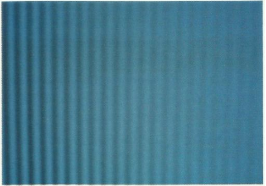
\includegraphics[width=0.3\textwidth]{./img/OMPPrectilgne.png}
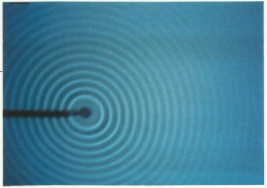
\includegraphics[width=0.3\textwidth]{./img/OMPPcirculaire.png}
    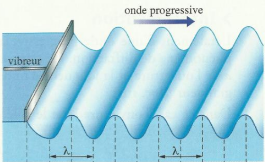
\includegraphics[width=0.3\textwidth]{./img/OMPPdemo.png}
\end{center}
\end{figure}


\subsection{Onde progressive à la surface de l'eau : }

On provoque une onde dans une cuve à onde par une source vibrante .Pour obtenir l'immobilité apparente on éclair la surface de l'eau par un stroboscope dont la fréquence est réglée sur une valeur égale à la fréquence de vibration de l'onde progressive c'est-à-dire celle de la source vibrante .On obtient par stroboscopie la figure suivante.


\begin{tcolorbox}

Toute onde périodique progressive présente une double périodicité:
  
une périodicité temporelle de période T;
  
une périodicité spatiale de période,appelée longueur d'onde.
\end{tcolorbox}

\subsubsection{Application 1:}
Sachant que la célérité de propagation de l’onde est $v=2,5m/s$ et la longueur de l’onde progressive est
$\lambda = 1cm$. Quelle est la fréquence de vibration de la source?


\subsubsection{Application 2:}
Dans l’expérience précédente, sachant que la plus grande fréquence du stroboscope qui permet d’obtenir l’immobilité apparente
est 250Hz.

En mesurant la longueur de l'onde progressive on obtient $\lambda=0.8cm$.

a) Quelle est la fréquence de l’onde progressive ? Justifier votre réponse.

b) Déterminer la célérité de propagation de l’onde progressive.

\subsection{Ondes sonores et ultrasonores : }
\begin{tcolorbox}
a - Les ondes sonores:
Les ondes sonores sont des ondes mécaniques périodiques longitudinales résultant de la compression et la dilatation des
constituants du milieu de propagation.
\end{tcolorbox}

\begin{tcolorbox}
b -Les ondes ultrasonores sont des ondes sonores dont la fréquence est supérieure à 20kHz, ils sont inaudibles et ils se réfléchissent
partiellement sur un obstacle.

(les ultrasons ne sont pas entendus par l’homme mais certains animaux comme les chauves souris, les dauphins ou les baleines
sont capable de les percevoir.)

\end{tcolorbox}


%*********************************************************************************************************
%\begin{wrapfigure}[10]{r}{0.5\textwidth}
%    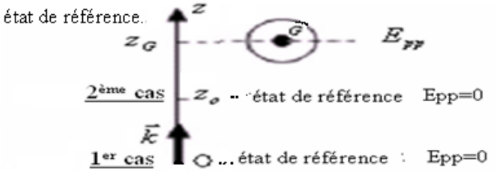
\includegraphics[width=0.5\textwidth]{./img/img00.png}
%\end{wrapfigure}

%\begin{center}
   %\begin{tabular}{ |c|c|c|c|c|c|c| }
      %\hline
      %km & hm & dam & \bf{m} & dm & cm & mm \\
      %\hline
        %&   &    &  &   &   & \\
%\hline
%\end{tabular}
%On place un seul nombre dans chaque case.
%\end{center}
%\begin{center}
   %\begin{tabular}{ |c|c|c|c|c|c|c| }
      %\hline
      %$km^2$ & $hm^2$ & $dam^2$ & \bf{$m^2$} & $dm^2$ & $cm^2$ & $mm^2$ \\
      %\hline
        %&   &    &  &   &   & \\
%\hline
%\end{tabular}
%\end{center}


\end{document}

